%%%% Paramétrage du TD %%%%
\def\xxactivite{Révisions \ifprof -- Corrigé \else \fi} % \normalsize \vspace{-.4cm}
\def\xxauteur{\textsl{Xavier Pessoles}}


\def\xxnumchapitre{Révision 1 \vspace{.2cm}}
\def\xxchapitre{\hspace{.12cm} Résolution des problèmes de statique -- Statique 2D}
\def\xxonglet{\textsf{Rév -- Stat}}
\def\xxactivite{TD 01}
\def\xxauteur{\textsl{Xavier Pessoles}}

\def\xxpied{%
Révision statique -- Résolution des problèmes de statique plane\\
Fiche 1 -- \xxactivite%
}

\def\xxcompetences{%
\vspace{-.3cm}
\textsl{%
\textbf{Savoirs et compétences :}\\
%\vspace{-.4cm}
%\begin{itemize}[label=\ding{112},font=\color{ocre}] 
%%\item \textit{Res1.C4 : } Correction
% \item \textit{Res1.C4.SF1 : } Proposer la démarche de réglage d’un correcteur proportionnel
%%proportionnel intégral 
%%et à avance de phase
%\item \textit{Con.C2 : } 	Correction d’un système asservi	
%\item \textit{Con.C2.SF1 : } Choisir un type de correcteur adapté
%\end{itemize}
}}

\def\xxauteur{\textsl{Xavier Pessoles}}

\def\xxtitreexo{Modélisation d'un hayon de coffre électrique}
\def\xxsourceexo{\hspace{.2cm} \footnotesize{Concours Centrale Supelec TSI 2013}}

\def\xxfigures{
\includegraphics[width=.55\textwidth]{fig_00}
}%figues de la page de garde


\iflivret
\input{style/new_pagegarde}
\else
\input{style/new_pagegarde}
\fi
\setlength{\columnseprule}{.1pt}

\pagestyle{fancy}
\thispagestyle{plain}

\vspace{5cm}

\def\columnseprulecolor{\color{ocre}}
\setlength{\columnseprule}{0.4pt} 

\setcounter{exo}{0}

%\ifprof
%%\begin{multicols}{2}
%\else
%\begin{multicols}{2}
%\fi
%%%%%%%%%%%%%%%%%%%%%%%%%%%%%%%%%%%%%%%%%%%%%%%%%%


\section{Les graphes ? Où ça ?}
Réseau de transport, Graphes du web, 
réseaux sociaux, bio-informatique. 

\section{Arbres binaires}

\begin{defi}[Arbres]\cite{ref_01}
Un arbre est un ensemble de \textbf{n\oe{}uds}, organisés de façon hiérarchique, à partir d'un n\oe{}ud distingué appelé racine. Les n\oe{}uds sont reliés entre eux par des arcs ou par des arrêtes. 
\end{defi}


\setlength{\columnseprule}{0pt}

\begin{multicols}{2}
\begin{figure}[H]
\centering
% définition des styles
\tikzstyle{lien}=[->,>=stealth,rounded corners=5pt,thick]
\tikzset{equipe/.style={draw,thick,fill=#1!25},
equipe/.default={white}}

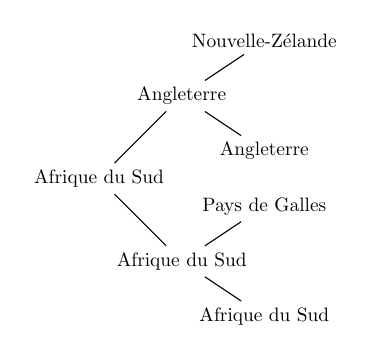
\begin{tikzpicture}[grow=right,scale=.7, every node/.style={scale=0.7},
level 1/.style={sibling distance=3cm},
level 2/.style={sibling distance=2cm},
%level 2/.style={level distance=3cm},
%level 3/.style={sibling distance=2cm},
%level 3/.style={level distance=1cm}
]
\node {Afrique du Sud} 
	child{ node  {Afrique du Sud}
		child { node  {Afrique du Sud} 
			%child { node {Afrique du Sud}}
			%child { node {Japon}}
		}
		child { node {Pays de Galles}
			%child { node {Pays de Galles}}
			%child { node {France}}
			}
		}
	child { node {Angleterre}
		child { node {Angleterre} 
			%child { node {Angleterre}}
			%child { node {Australie}}
			}
		child { node {Nouvelle-Zélande} 
			%child { node {Angleterre}}
			%child { node {Australie}}
				}
};
\end{tikzpicture}
\centering
\captionsetup{justification=centering}
\caption{Dernier carré du Championnat du monde de Rugby à XV 2019}
\end{figure}


\begin{figure}[H]
\centering
% définition des styles
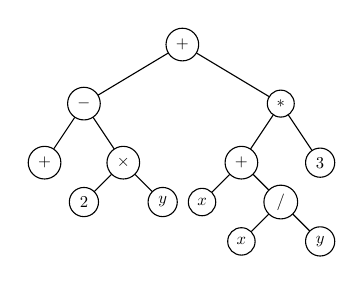
\begin{tikzpicture}[scale=.5, every node/.style={scale=0.6},
level 1/.style={sibling distance=5cm},
level 2/.style={sibling distance=2cm},
%level 2/.style={level distance=3cm},
%level 3/.style={sibling distance=2cm},
level 3/.style={sibling distance=2cm},
level 4/.style={sibling distance=.8cm},
level 3/.style={level distance=1cm},
level 4/.style={level distance=1cm},
]
\node [circle,draw]  {$+$} 
	child{ node [circle,draw]  {$-$}
		child { node [circle,draw]  {$+$}}
		child { node  [circle,draw] {$\times $}
			child { node [circle,draw]{2}}
			child { node [circle,draw]{$y$}}
			}
		}
	child { node [circle,draw]{$*$}
		child { node [circle,draw]{$+$} 
			child { node [circle,draw]{$x$}}
			child { node [circle,draw]{$/$} 
				child { node [circle,draw] {$x$}}
				child { node [circle,draw]{$y$}}
				}
			}
		child { node [circle,draw] {$3$} }
};
\end{tikzpicture}
\captionsetup{justification=centering}
\caption{Arbre codant l'expression arithmétique $(x-2\times y)+\left(x+y/z\right)\times 3$}
\end{figure}

\end{multicols}

\begin{defi}[Arbre binaire]\cite{ref_03}

Un arbre binaire est un arbre pour lequel chaque n\oe{}uds a au plus deux fils.

Un n\oe{}ud n'ayant pas de fils est appelé \textbf{feuille}. 

Le niveau d'un nœud, autrement dit la distance entre la feuille la plus éloignée et la racine, est appelé \textbf{profondeur}.
\end{defi}


Les arbres ci-dessus sont des arbres \textbf{binaires}, c'est-à-dire que chaque n\oe{}uds a au plus deux fils. 


\begin{defi}
Un arbre binaire (ou binaire-unaire) est un arbre avec une racine dans lequel chaque nœud a au plus deux fils.

Un arbre binaire strict ou localement complet est un arbre dont tous les nœuds possèdent zéro ou deux fils.

Un arbre binaire dégénéré est un arbre dans lequel tous les noeuds internes n'ont qu'un seul fils. Ce type d'arbre n'a qu'une unique feuille et peut être vu comme une liste chaînée.

Un arbre binaire parfait est un arbre binaire strict dans lequel toutes les feuilles (nœuds n'ayant aucun fils) sont à la même distance de la racine (c'est-à-dire à la même profondeur). Il s'agit d'un arbre dont tous les niveaux sont remplis: où tous les noeuds internes ont deux fils et où tous les noeuds externes ont la même hauteur.

Un arbre binaire complet ou presque complet, à ne pas confondre avec localement complet (ci-dessus), est un arbre dans lequel tous les niveaux sont remplis à l'exception éventuelle du dernier, dans lequel les feuilles sont alignées à gauche. On peut le voir comme un arbre parfait dont le dernier niveau aurait été privé de certaines de ses feuilles en partant de la plus à droite. Une autre façon de le voir serait un arbre binaire strict dans lequel les feuilles ont pour profondeur n ou n-1 pour un n donné. Le caractère éventuel est important: un arbre parfait est nécessairement presque complet tandis qu'un arbre presque complet peut être parfait.
\end{defi}

\subsection{Une première implémentation}

\begin{figure}[H]
\centering
% définition des styles
\begin{tikzpicture}[
%scale=.5, every node/.style={scale=0.6},
level/.style={sibling distance=60mm/#1},
%level 1/.style={sibling distance=5cm},
%level 2/.style={sibling distance=2cm},
%level 2/.style={level distance=3cm},
%level 3/.style={sibling distance=2cm},
%level 3/.style={sibling distance=2cm},
%level 4/.style={sibling distance=1cm},
%level 3/.style={level distance=1cm},
%level 4/.style={level distance=1cm},
]
\node [circle,draw] {A} 
	child{ node  [circle,draw] {B}
		child { node [circle,draw] {D}}
		child { node [circle,draw] {E}
			child { node [circle,draw] {F}}
			%child { node {$y$}}
			}
		}
	child { node [circle,draw]  {C}
		child { node  [circle,draw] {G} 
			%child { node {$x$}}
			%child { node {$/$} 
				%child { node {$x$}}
				%child { node {$y$}}
				%}
			}
		%child { node {$3$} }
};
\end{tikzpicture}
\captionsetup{justification=centering}
\caption{Arbre codant l'expression arithmétique $(x-2\times y)+\left(x+y/z\right)\times 3$}
\end{figure}


\begin{lstlisting}[language=python]
>>> graph = {'A': ['B', 'C'],
             'B': ['D', 'E'],
             'C': ['G'],
             'D': [''],
             'E': ['F'],
             'F': ['']
             'G': [''],}
    
\end{lstlisting}

\section{}
\begin{defi}[Graphe orienté]

\end{defi}

\begin{defi}[Graphe non orienté]

\end{defi}

\begin{defi}[Sommet -- n\oe{}ud]

\end{defi}

\begin{defi}[Arc]

\end{defi}


\begin{defi}[Arête]

\end{defi}


\begin{defi}[Boucle]

\end{defi}


\begin{defi}[Degré entrant et sortant]

\end{defi}



\begin{defi}[Chemin d'un sommet à un autre]

\end{defi}


\begin{defi}[Cycle]

\end{defi}


\begin{defi}[Connexité dans les graphes non orientés]

\end{defi}







\ref{01}{Types de données algorithmes, Christine Froidevaux, Marie-Christine Gaudel, Michèle Soria. Mc Graw -- Hill.}

\ref{02}{\url{https://www.python.org/doc/essays/graphs/}}

\ref{03}{\url{https://fr.wikipedia.org/wiki/Arbre_binaire}}
